\documentclass[12pt,a4paper]{report}

\usepackage{cite}
\usepackage{amsmath}
\usepackage{amssymb}
\usepackage{amsfonts}
\usepackage{graphicx}
\usepackage{textcomp}
\usepackage{xcolor}
\usepackage{makeidx}
\usepackage{tocbibind}
\usepackage{setspace}
\usepackage{lipsum}
\usepackage{footmisc}
\usepackage{algpseudocode}
\usepackage{url}
\usepackage{algorithm}
\usepackage{float}
\usepackage{hyperref}
\hypersetup{
    colorlinks=true,
    linkcolor=black,
    filecolor=magenta,
    urlcolor=cyan
}

\begin{document}

\renewcommand\bibname{References}

\chapter*{Abstract}
The whole aim of this project is to tackle the problem of communication between deaf and dumb people with computers using a standard sign language system called ISL(Indian Sign Language) as the common medium of communication on either side. This project can be used to assist them in conversing with computers in a better way by allowing them to use sign language to fill forms or input text in the computer. The project is basically a model which takes a static image input showing an ISL hand sign and tries to predict the characters which closely match the ISL signs shown in the static image by using Mediapipe and a neural network to classify the character shown in the image. This way we can predict characters and numbers which can be further passed through a NLP(Natural Language Processing) medium to tokenize the stream of characters into words and spellcheck each and every word to get the correct sentence which the user wants to interpret. This final sentence formed can be used to converse with a chat bot by selecting its options and entering text when required. We also created a model and its working architecture keeping in mind that the model and its architecture is very fast in terms of predictions and is fully scalable to serve a large number of users so that it can be deployed in real time as a chatbot interface to make it easy to access and use.

\tableofcontents
\listoffigures
\listoftables

\chapter{Introduction}

\section{Problem Statement}
Our problem statement is to basically create a chatbot which interacts with deaf and dumb people using a common medium as ISL(Indian Sign Language) so that the person can show ISL hand signs to enter text which can be used to fill forms or select options which provides them a better way to interact with the computer. We also have to address the problem of fast predictions and scaling of this chatbot to serve to multiple users at a time on a very light weight architecture.

\section{Motivation}
In today's world, deaf and dumb people have a hard time communicating with others and this this becomes even more harder if it is a computer as the deaf and dumb person most likely does not know how to operate a computer and most of the services today like payments, purchasing and customer support are computerized making it a lot harder for them to use these services. Hence it becomes increasing difficult for dumb people to interact with the computer and to make things worse, they cannot use the customer support since they are dumb and deaf and have no way to converse with the support. Hence this project aims at creating a way for deaf and dumb people to converse with computers by using a common medium of ISL(Indian Sign Language).

\section{Objectives}
The main objectives addressed in this project are:-
\begin{itemize}
	\item Create a web interface based chatbot where in we take webcam feed of the deaf and dumb user so that he can interact with the computer and show ISL hand signs which can be used to input text in input fields or select options for him in any forms or any kind of interface in the computer.
	\item Provide a NLP(Natural Language Processing) mechanism which can be used to add spaces to raw predictions which are words clubbed without spaces and spellcheck words.
	\item Make the chatbot scalable across for multiple users.
	\item The architecture needs to be as fast and seamless as possible.
\end{itemize}

\section{Contribution}
Our contributions to this project are:-
\begin{itemize}
	\item 2 different models for predicting ISL hand signs in an image.
	\item Special preprocessing function in case of CNN model for getting borders of image based on erosion and dialation.
	\item Special preprocessing function in case of mediapipe based model for transforming and translating hand coordinates.
	\item A Web UI based chatbot with frontend and backend for running the model.
	\item NLP techniques for spellchecking and word segmentation for the chatbot.
	\item OpenCV based UI for testing the model in realtime with webcam feed.
	\item Scalable architecture for making the chatbot work for multiple users.
\end{itemize}

\section{Indian Sign Language}
Indian Sign Language (ISL) is used in the deaf community all over India. It is a way of conversing with other people without speaking by showing hand signs which represent characters(alphabets or numbers). In the past years, there has been an increased interest among researchers in the field of sign language recognition. One of which is to introduce means of interaction from human to computer. Deaf and Dumb people generally rely on sign language interpreters for communication. Finding experienced and qualified interpreters for their daily communication throughout life is a very difficult task and also unaffordable. Hence, a human to computer interaction system will prove to be a reliable and consistent solution in the future for deaf and dumb people.The ISL has different hand sign for each character so that a person can show these hand signs to spell out the word they want to convey or the sentence they want to convey to others. Now this medium has been used by us in this project as a common medium between the user and computer for conversing since most of the deaf people generally use this sign language to converse with each other.
\begin{figure}[htbp]
	\centerline{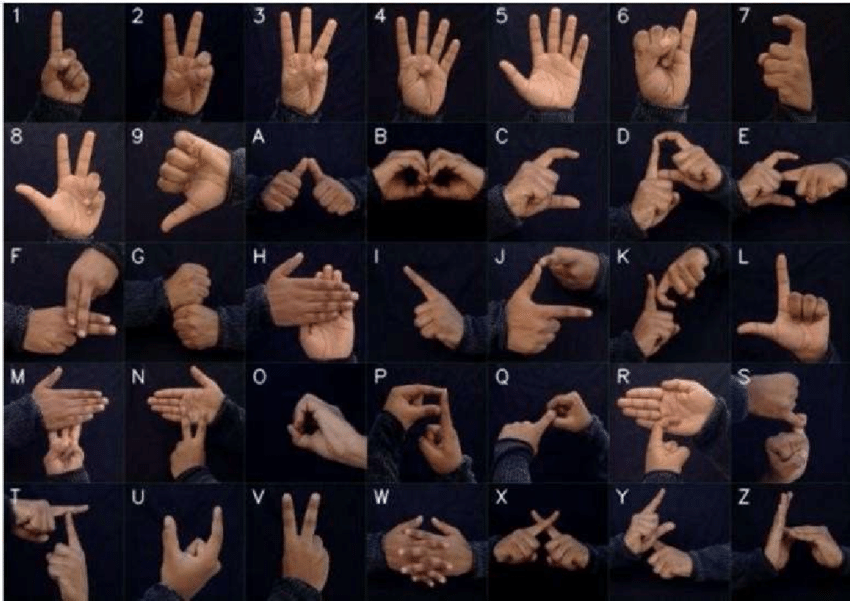
\includegraphics[scale=1]{isl.png}}
	\caption{ISL Hand Signs}
	\label{Isl}
\end{figure}
\begin{figure}[htbp]
	\centerline{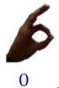
\includegraphics[scale=1]{isl_0.png}}
	\caption{ISL Hand Sign for 0}
	\label{Isl0}
\end{figure}

\chapter{Models, Architecture and Proposed Frameworks}

\section{Preamble}
This chapter explains about various models tested for our chatbot purpose. It gives us an insight of various frameworks used in our project. It also helps us understand the whole architecture employed for the chatbot to work flawlessly. It also tells us about the special preprocessing techniques used on the input in the case of various models tested for our chatbot.

\section{Literature Review}

\subsection{Sign Language Recognition for Static and Dynamic Gestures by Jay Suthar\cite{b1}}
This paper proposes two methods for recognizing hand gestures. Static gestures and dynamic gestures. For static gesture classification, a CNN model is implemented that classifies alphabets and numbers shown in ISL in a photo with a accuracy percentage of 73. For dynamic gestures a model using multi-layer LSTM using 12 word MobileNetV2 and gave very satisfactory results with an accuracy percentage of 85.

\subsection{Zero-Shot Sign Language Recognition: Can Textual Data Uncover Sign Languages? by Yunus Can Bilge\cite{b2}}
This study presented the challenge of zero-shot sign language recognition (ZSSLR), which aims to detect instances of unseen signs by leveraging models developed from visible sign class samples. They proposed a system that uses sign language dictionaries' readily available descriptions as an intermediate-level semantic representation for knowledge transfer, as well as a framework that operates over the body and hand regions using 3D-CNNs and models longer temporal relationships using bidirectional LSTMs. Using descriptive text embedding in conjunction with these Spatial-temporal representations within a zero-shot learning framework shown that textual data may be effective in discovering sign languages.

\subsection{A Review Paper on Sign Language Recognition of Engineering System For Deaf And Research \& Dumb People using Image Technology Processing by Manisha U. Kakde\cite{b3}}
The paper goes into detail about the various types of "automatic sign converter tool" and their various hardware and software features. The research concentrates on two types of sign language recognition. Glove-based and image-processing-based systems.

\subsection{Attention-Based Sign Language Recognition Network Utilizing Key frame Sampling and Skeletal Features by Wei Pan\cite{b4}}
This work enhanced keyframe centered clips (KCC) sampling to provide a new type of sampling approach known as optimized keyframe-centered clips (OptimKCC) sampling for selecting important actions from sign language films. To characterize the video clips, they created a new type of skeletal feature called Multi-Plane Vector Relation (MPVR). Finally, they integrated the attention mechanism with extracted vector attention-based networks to distribute weights to temporal and spatial information taken from skeletal data. They also carried out comparative studies on their own and the public sign language dataset under Signer-Independent and Signer-Dependent conditions to demonstrate the benefits of our approaches.

\section{Methodology, Architecture and Proposed Frameworks}

\subsection{Architecture}
\begin{figure}[htbp]
	\centerline{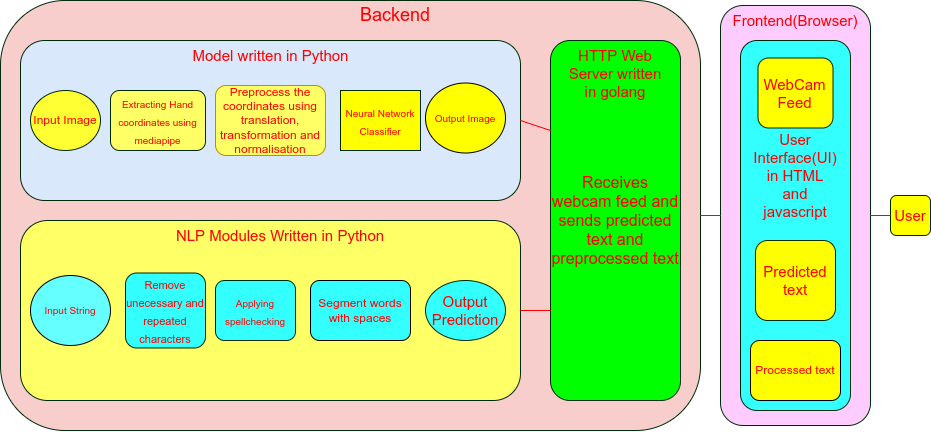
\includegraphics[scale=0.4]{architecture.png}}
	\caption{Chatbot Architecture}
	\label{Architecture}
\end{figure}
When the user accesses the chatbot from the frontend, he provides the webcam feed to it in which he shows the hand sign. Now this frame is sent to the backend which then sends it to the python prediction model. When the model receives the image, it first extracts the hand coordinates from the image using mediapipe and then passes it to a special preprocessing function which translates and transforms the coordinates and sends to the the actual neural network classifier which then gives an output as to which character was shown in the image. Now this predicted character is passed back to the backend ny the python prediction model which then passes it to the frontend. If the user is inputting a word and he wants to correct the spelling, then we can enable spellchecking for that entered word to get it autocorrected. When spellchecking is enabled, the frontend will send the incorrect word to the backend which sends the incorrect word to the pyspellchecker based python NLP module which returns back the correct spelling to the backend which is then returned back to the frontend by the backend. In the same way, this also applies if we want word segmentation in case we are inputting sentences instead of words.

\subsection{Using Inception-ResNet-v2 convolutional neural network (CNN) pre-trained model to detect hand signs in the image}
\begin{figure}[htbp]
	\centerline{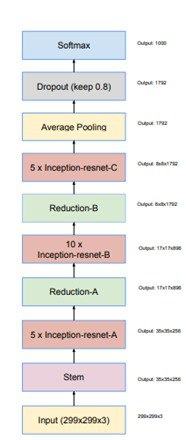
\includegraphics[scale=0.5]{cnn.jpg}}
	\caption{CNN model architecture}
	\label{Cnn}
\end{figure}
Deep convolutional networks have been at the heart of the most significant breakthroughs in image recognition performance in recent years. The Inception design, for example, has been proven to deliver extremely excellent performance at a cheap computational cost. Recently, the use of residual connections in combination with a more conventional design produced state-of-the-art performance in the 2015 ILSVRC challenge, comparable to the current generation Inception-v3 network. This begs the issue of whether combining the Inception design with residual connections is beneficial. We show here that training using residual connections considerably speeds up the training of Inception networks. In addition, there is some evidence that residual Inception networks outperform comparably priced Inception networks without residual connections by a narrow margin. In addition, we offer various novel simplified designs for residual and non-residual Inception networks. The Inception-ResNet-v2 convolutional neural network was trained on over a million photos from the ImageNet collection. The network has 164 layers and can identify photos into 1000 item categories, including keyboards, mice, pencils, and a variety of animals. As a consequence, the network has learnt detailed feature representations for a diverse set of pictures. The network's picture input size is 299 by 299 pixels. In this approach a CNN model is trained specifically inceptionresnetv2 with the given dataset and the aim is to try to increase its accuracy by making minor tweaks to the model. After trying out many popular CNN classifiers like ShuffleNet and different versions of ResNet it turns out that InceptionResNet outperformed these models and gave good accuracy both in training and testing when compared to all other models. So basically in this architecture, we pass the image directly to the CNN and make it predict which character's ISL hand sign of the 36 characters is shown in the image and get the output.

\subsubsection{Using erosion and dialation to get all the borders in the picture}
\begin{figure}[htbp]
	\centerline{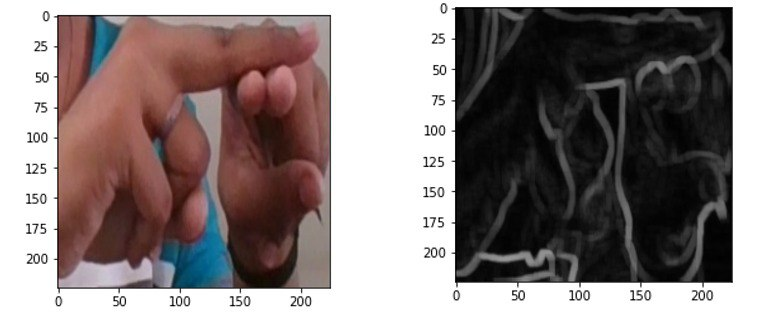
\includegraphics[scale=0.5]{erosion_dialation.jpg}}
	\caption{Erosion and Dialation of a image}
	\label{Erosion_dialation}
\end{figure}
This is a special image processing technique which was later used as the preprocessing function for the dataset passed to the CNN to get a little bit better accuracy. We will first erode and dilate the given image and subtract the eroded image from the dilated which will result in an black and white image consists of edges in white and the background in black. This technique is useful for detecting the shape of the hand which is very crucial feature for the classifier model to consider and helps in making the model not focus on other parameters like color of the hand, background, etc. But the issue with this approach was that it still returned edges of other objects with the hands.

\subsection{Using MediaPipe to get hand coordinates in the image and pass them to a neural network classifier to detect hand signs in the image}
Perception of hand shape and motion may be a critical component in improving user experience across a wide range of technical disciplines and platforms. It can, for example, serve as the foundation for sign language comprehension and hand gesture control, as well as enabling the overlay of digital material and information on top of the actual environment in augmented reality. While it comes naturally to people, robust real-time hand perception is a difficult computer vision task because hands frequently occlude themselves or each other (e.g., finger/palm occlusions and handshakes) and lack high contrast patterns. MediaPipe Hands is a solution for high-fidelity hand and finger tracking. Machine learning (ML) is used to deduce 21 3D landmarks of a hand from a single shot. Whereas existing state-of-the-art algorithms for inference rely mostly on powerful desktop settings, our method provides real-time performance on a mobile phone and even scalable to several hands. MediaPipe development team anticipate that making this hand perception capabilities available to the broader research and development community will spark the creation of new applications and research fields. In this approach we passed the static image through a framework called MediaPipe created by google which can detect 21 3-dimensional landmarks of a hand in a given picture and get the landmarks of both hands. These landmarks of both the hands which are detected and given by MediaPipe are passed through a custom neural network classifier that predicts which character is being shown based on the hand coordinates given. Altough we first used 3-dimensional landmarks, at a later stage we started considering only 2-dimensional landmarks since the third dimension was redundant since hand shapes were all that mattered in ISL hand signs.
\begin{figure}[htbp]
	\centerline{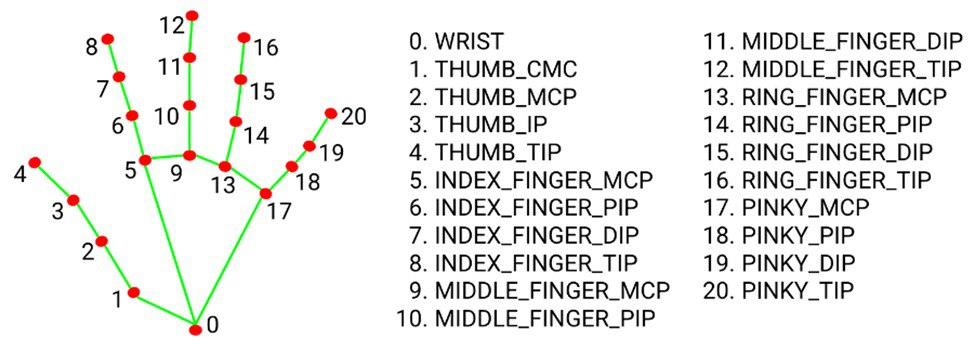
\includegraphics[scale=0.3]{mediapipe.jpg}}
	\caption{Mediapipe hand coordinates}
	\label{Mediapipe}
\end{figure}
\begin{figure}[htbp]
	\centerline{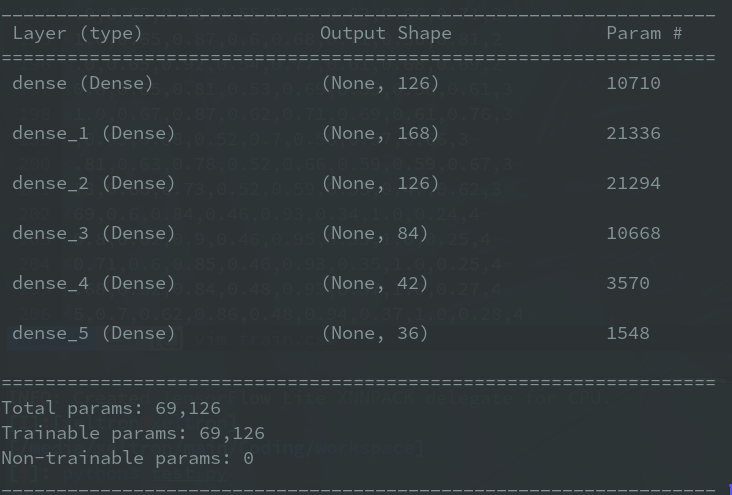
\includegraphics[scale=0.5]{neural_network.png}}
	\caption{Neural Network Architecture}
	\label{Neural_net}
\end{figure}

\subsubsection{Transforming, translating and normalising the coordinates}
Initially we weren't getting good accuracy with ISL hand signs in the image in the case of mediapipe based neural network classifier during runtime due to the following reasons:-
\begin{itemize}
	\item If the hand was too close the camera it was bigger in size in the picture and if the hand was too far away from the camera it was smaller in size in the picture.
	\item Also there are ISL hand signs which require both hands to make the hand sign. These hand signs become difficult to predict because sometimes the user might show both hands closely when making the ISL hand sign while other times he might show them a bit away from each other while making the ISL hand sign.
\end{itemize}
To address this issue we use the following formulae to transform and translate the hand coordinates so that the neural network can train well on the data and give better performance in real time.
\begin{itemize}
	\item This equation is applied on the coordinates of each hand seperately so as to translate and transform it to a range between 0 to 100 regardless of it previous position. This ensures that the hand is of same size even if it is bigger or smaller in the image. It also removes the relativity of positions between both the hands since all we need to consider are the hands shapes and not their positions with respect to each other.
	      \begin{equation}
		      Transformed\ Value = \frac{Actual\ Value - Min\ Value}{Max\ Value - Min\ Value} \notag
	      \end{equation}
	\item This equation is applied on the coordinates of both hands to bring them to a range between 0 and 100. This is just an intermediate step which is done to remove extra decimal points and is the first step of normalisation.
	      \begin{equation}
		      Scaled\ Value = Transformed\ Value * 100 \notag
	      \end{equation}
	\item This equation is applied to remove decimal points from the coordinates of both hands in a range between 0 and 100 and bring them back to a range between 0 and 1. This effectively makes sure that only 2 decimal points are there in all coordinates before passing them to the neural network. This is the second step of normalisation.
	      \begin{equation}
		      Normalised\ Value = \frac{|Scaled\ Value|}{100} \notag
	      \end{equation}
\end{itemize}

\subsection{NLP}
Our final output from the model will be one of the (26 letters + 10 numbers)36 characters or an "-"(nothing predicted in case the model's confidence rate is less than 95\%) as prediction from the model. But in realtime it will not just be one image but a stream of continuous frames and the raw output from the model will be concatenated to a string of characters altought "-" predictions are not concatenated. This string needs to be processed in order to make meaningful word or sentence. For processing the model's raw output string we introduced three approaches.

\subsubsection{Taking the element with maximum frequency across some samples}
So the output we deal with will be something like "CCCCAACCAA" if we are trying to show a the ISL hand sign for the character "C" for 10 frames with some misclassifications. To address this issue, we take a sample size of 10 by default and for every ten frames from the webcam we get the predictions string for 10 characters from the model and then only take the maximum occurring character in the ten frames which is predicted by the model as the character which the user wanted to convey. For better understanding let us take the sample string "CCCCAACCAA" for reference from above, since "C" is the maximum occuring character, that is taken as the input character which the user wanted to convey. In this way we try to reduce error in predictions and finally all the predictions here are appended to a string which will undergo further NLP processing.

\subsubsection{Spellchecking}
Lets just say the user tried to predict the word "CAB" but it turned out to be "CLB". In that case we use a spellchecking module in python called "pyspellchecker" module which uses to NLP technique to correct this word to "CAB". The NLP technique it uses is Levenshtein Distance algorithm. It uses this algorithm to find the permutations within edit distance of 2 from the original word. Simply said, it can correct words which have about 2 characters wrong in its spelling to right ones. This way we can correct spelling mistakes in the word so that the actual word can be used as input.

\subsubsection{Word Segmentation}
Lets just say the user tried to use the model to predict a sentence like "HOW ARE YOU". The model's output will be something like "HOWAREYOU". Essentially speaking there are no spaces here since ISL has so sign for a space character which is a special character. So we used another python based NLP module called "wordsegment" which essentially uses words from Google Web Trillion Word Corpus data which are the most common words to segment words in a sentence. Simply said it can seperate words which are clubbed in a sentence without spaces as long as they are within its dataset of the most commonly used words.

\subsection{Chatbot}

\subsubsection{Frontend}
Since our goal is for the chatbot to work as fast as possible, we went ahead and built the frontend without using any external frontend framework and just commonjs so that it works fast. We also made the code run as asynchronously as possible so that there wont be any blocking calls in code which take lot of time to resolve thus slowing down the whole chatbot process making it slower in predictions. In this way we made sure everything works as fast as possible from the frontend side so that the user can have a seamless UI experience. We capture the webcam feed of the user in the frontend and also predict if his hands are being shown in the image with the help of mediapipe framework and notify the user if his left hand, right hand or both are not visible in the feed additionally along with predicting characters so that the user can know if the model is able to detect his hand and change his background if his hands blend in the background or move his hand to a better position so that the hand is visible in the image.
\begin{figure}[htbp]
	\centerline{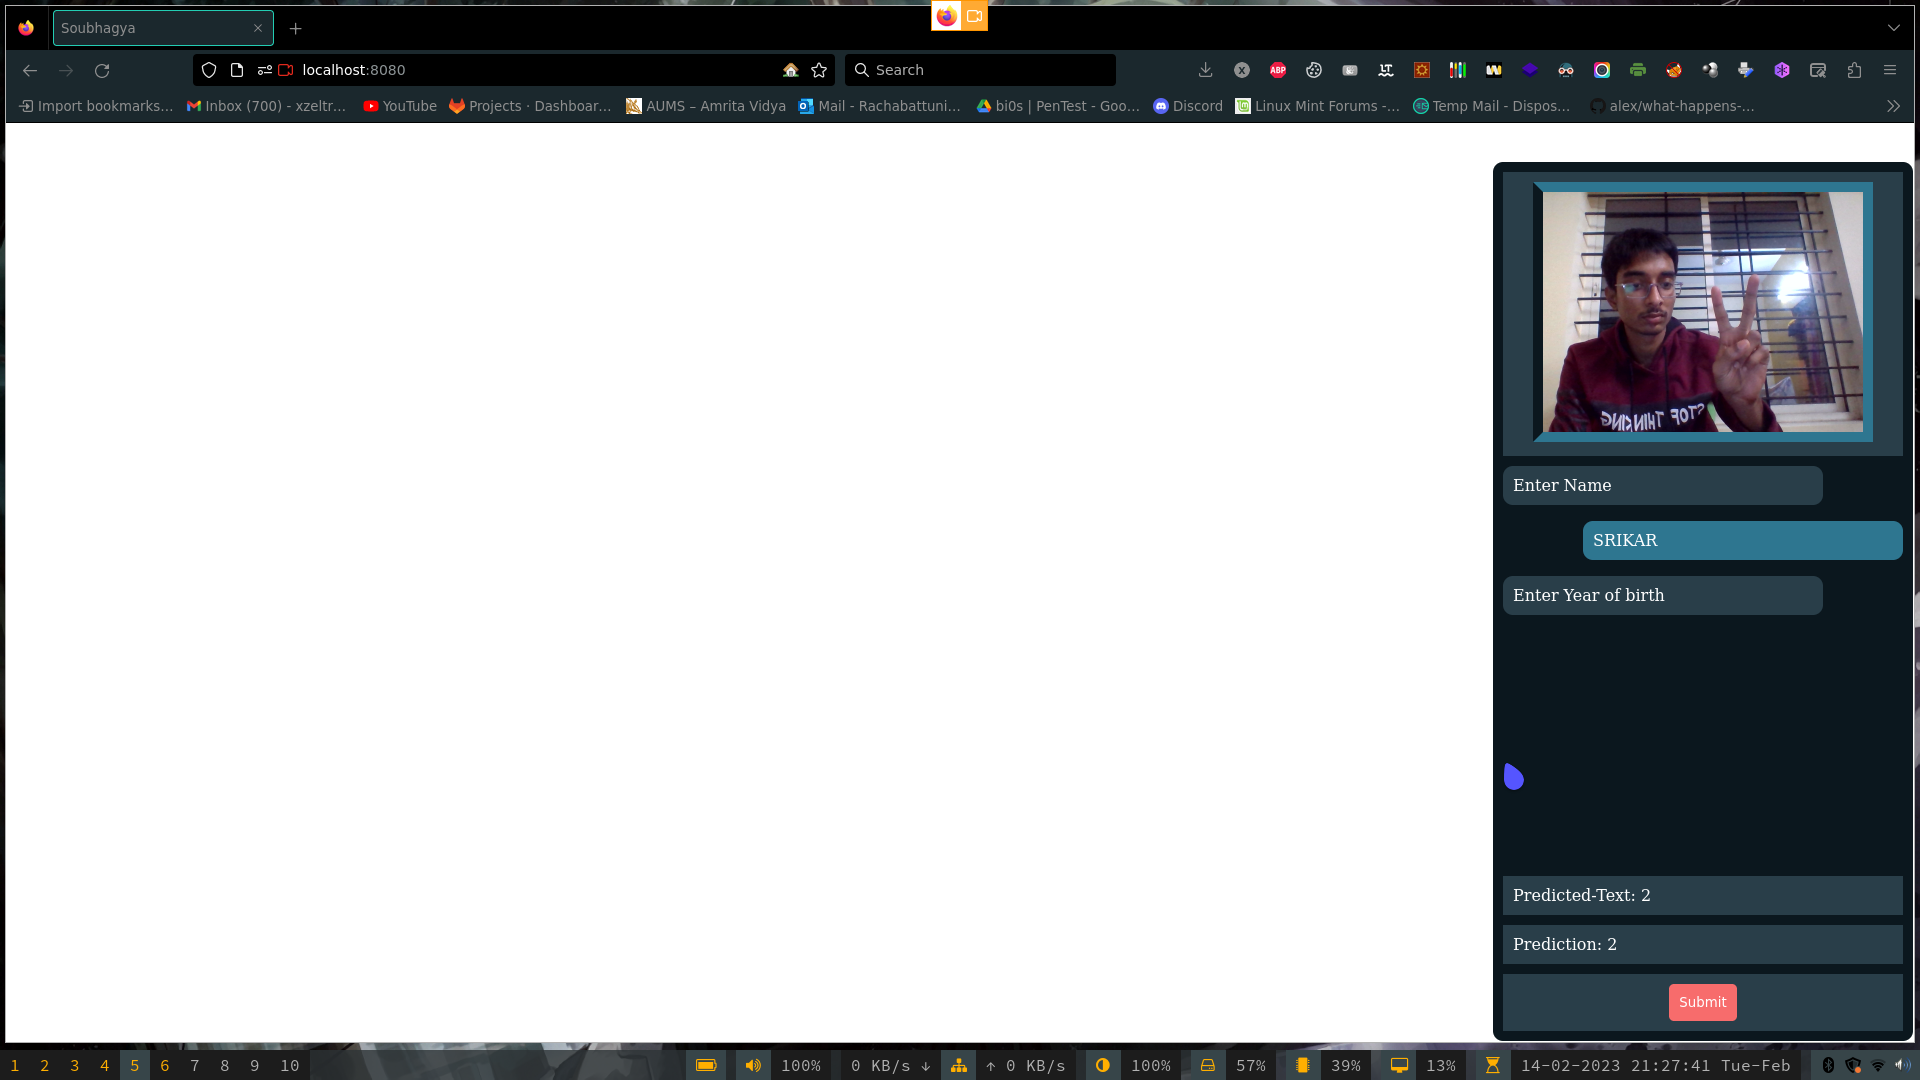
\includegraphics[scale=0.2]{ui.png}}
	\caption{chatbot frontend}
	\label{ui}
\end{figure}

\subsubsection{Backend}
On the backend side, we used Golang for writing our http server. We went with golang since it is a compiled language and faster than python and javascript which are interpreted languages. We also did not want to go with java since JRE(Java Runtime Environment) is required for the build to work in this case and also java is slower than golang. Golang handled multitasking well using the concept of concurrency which is implemented by goroutines in golang. Golang is also really fast at handling streams and file descriptors which will be useful in our case since we send all the frames which we capture in the frontend to the backend. It also supports cross platform builds like java which is a huge advantage if we want to deploy out server in a windows machine at a later stage. Our runtime working neural network classifier which is a python based tensorflow model is loaded as the server starts so as to not waste any time during predictions. We also use the concept of mutex locks which enables one model to predict characters for many users. This can be a huge difference as it reduces the amount of hardware required as if there was one model per user, it would take lot of computational power.

\subsubsection{Scaling the chatbot to serve for multiple users}
Finally, we have to scale the chatbot so that it works for multiple users so that it can be deployed in realtime. For this we dockerised the whole application and created a docker image which can be used to spawn many containers and manage them using kubernetes so that it can be deployed in realtime. We also programmed the backend in a way where each container is independent of the other so that any number of containers can be spawned without any issue.

\section{Results and Discussion}

\subsection{Experimentation Environment}

\subsubsection{CNN model training methods}
For the InceptionResNetV2 CNN model, we introduced hyper parameter tuning techniques like data augmentation, EarlyStopping, ReduceLROnPlateau, Class Balancing and custom data preprocessing which gave the best accuracy and improved the training process. We also tried changing with various neural network parameters like learning rate, batch size, optimizers, loss functions and no of epochs for best training results. We also tried the training with and without the erosion and dialation preprocessing function.

\subsubsection{Mediapipe based neural network classifier model training methods}
For this model, we tried changing experimenting with the neural network layers so as to finally land on the one model layer architecture which is the smallest, simple, easy to train and doesn't compromise on accuracy during training or testing time on a live webcam feed. We also tried training with various neural network parameters like learning rate, batch size, optimizers, loss functions and no of epochs for best training results. We also tried the training with and without the translation and transformation preprocessing function to check whether the accuracy is increasing or not.

\subsection{Dataset}

\subsubsection{Older dataset}
We had existing custom dataset which has average of 3000 images per class but has many problems such as imbalance in number of images per class which had led to good accuracy but low f1 score and missing digits (5 characters) out of 36 characters (26 alphabets and 10 digits) to solve these problems we had combine this data set with the popular ISL sign language data set from the Kaggle and did some data preprocessing to attain the balanced number of images per class. This dataset got good accuracy with both the CNN and mediapipe based neural network classifier models during training time. But during testing time, both the models performed badly since most of the images in the model were blurry and unclear. Also in the case of mediapipe based classifier, mediapipe couldn't detect the hands in some pictures while in some pictures, it detected the hands wrongly. This became a issue which haunts us during the testing phase with webcam feed.

\subsubsection{Newer dataset}
We created a custom dataset which stores 85(21*2(left hand) + 21*2(right hand) + 1(prediction)) values in a CSV(Comma Seperated Values) format. Each entry in it represents the hand coordinates and its respective prediction. Also note that these 84 coordinates are preprocessed using the special function to translate and transform hand coordinates before storing it in the file. The newer dataset consists of a total of 720 samples with 20 samples represent each class.

\subsection{Evaluation Metrics}
We have used Categorical Cross entropy Loss function for the both the models to computes the cross-entropy loss between the labels and predictions. This loss function is frequently employed in multi-class classification models with two or more output labels. We used Adam as the optimizer function for both the models since that was giving the best result for both the training models. We evaluated the model based on training and testing accuracy graphs. We also tested the models in realtime with webcam feed to check its accuracy.

\subsection{Results}
\begin{table}[h]
	\centering
	\begin{tabular}{ | c | c | c | c | }
		\hline
		Model                     & Accuracy & Loss  & Realtime \\
		\hline
		CNN                       & 99\%     & 0.1\% & Fails    \\
		Neural Network Classifier & 99\%     & 0.1\% & Passes   \\
		\hline
	\end{tabular}
	\caption{Model Comparision}
\end{table}

\subsubsection{CNN model}
Although the CNN model gave really high accuracy during training and testing, it couldn't not do the same in realtime with a webcam feed. Upon further research into why the model was failing, we found out that we had to do some kind of hand detection in the image since during realtime, the background is not plain all the time as it was in the training data. Also, we the hand might be closer or farther in the image making it bigger or smaller in the image respectively. Another reason is the relative positions of both hands with respect to each other during ISL hand signs as different people show hand signs in different relative hand positions. Also running a CNN model means that predictions are significantly slower as bit as resnet means that our predictions will gradually becomes slower which hinders our main objective which is to make predictions faster. Also complex ISL hand signs like "M" and "N" for example weren't being recoginzed at all. Since we had to address these many problems and also this slower predictions problem cannot be addressed in any way to make it faster we had to move away from this approach for predicting hand signs in the image.
\begin{figure}[htbp]
	\centerline{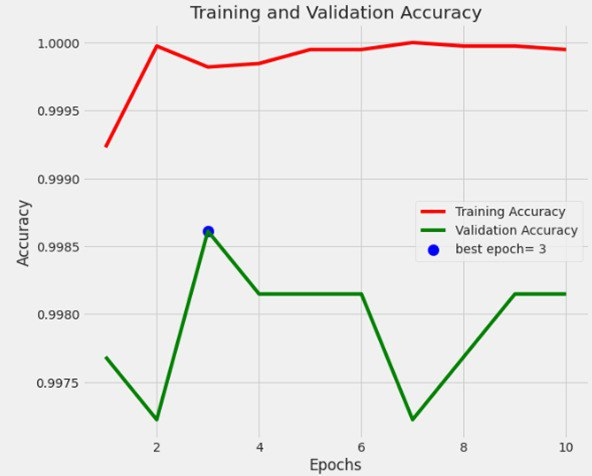
\includegraphics[scale=0.5]{cnn_accuracy.jpg}}
	\caption{CNN model accuracy}
	\label{Cnn_accuracy}
\end{figure}
\begin{figure}[htbp]
	\centerline{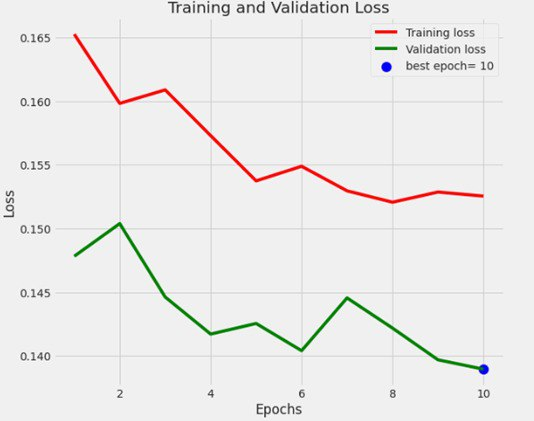
\includegraphics[scale=0.5]{cnn_loss.jpg}}
	\caption{CNN model loss}
	\label{Cnn_loss}
\end{figure}

\subsubsection{Mediapipe based neural network classifier model}
THis model as usual gave really high accuracy during training and testing but failed to give the same during runtime initially. After further research into this, we found out that the dataset we were using hand pictures in which mediapipe couldn't detect the hands or detected them incorrectly in many cases which lead to bad training. But it started giving better accuracy once we used the new dataset to train the model. But this time the issue is that the ISL hand signs are classified correctly only if we put the hands at the same distance from the camera as we put during the making of dataset as putting it nearer or farther than necessary would make them big or small in the image respectively. We also had this problem of relative positions of hands which differs for each person due to their hand size. We had to address the hands sizes and relative positions in the image and we did that using the special preprocessing function which translates and transforms all the hand coordinates to a range between 0 and 1 and removes the relativeness between the position of two hands as we only needed to know the shapes of the two hands to predict the image. Using this preprocessing function we were able to get really high training and testing accuracy and it was able to detect the ISL hand signs in realtime with a live webcam feed. This model could detect all the 36 characters including the complex ones in realtime without any hassle. Most of all this model was fast in terms of predictions. Hence we had to go forward with this model architecture for our predictions on ISL hand signs in the image.
\begin{figure}[htbp]
	\centerline{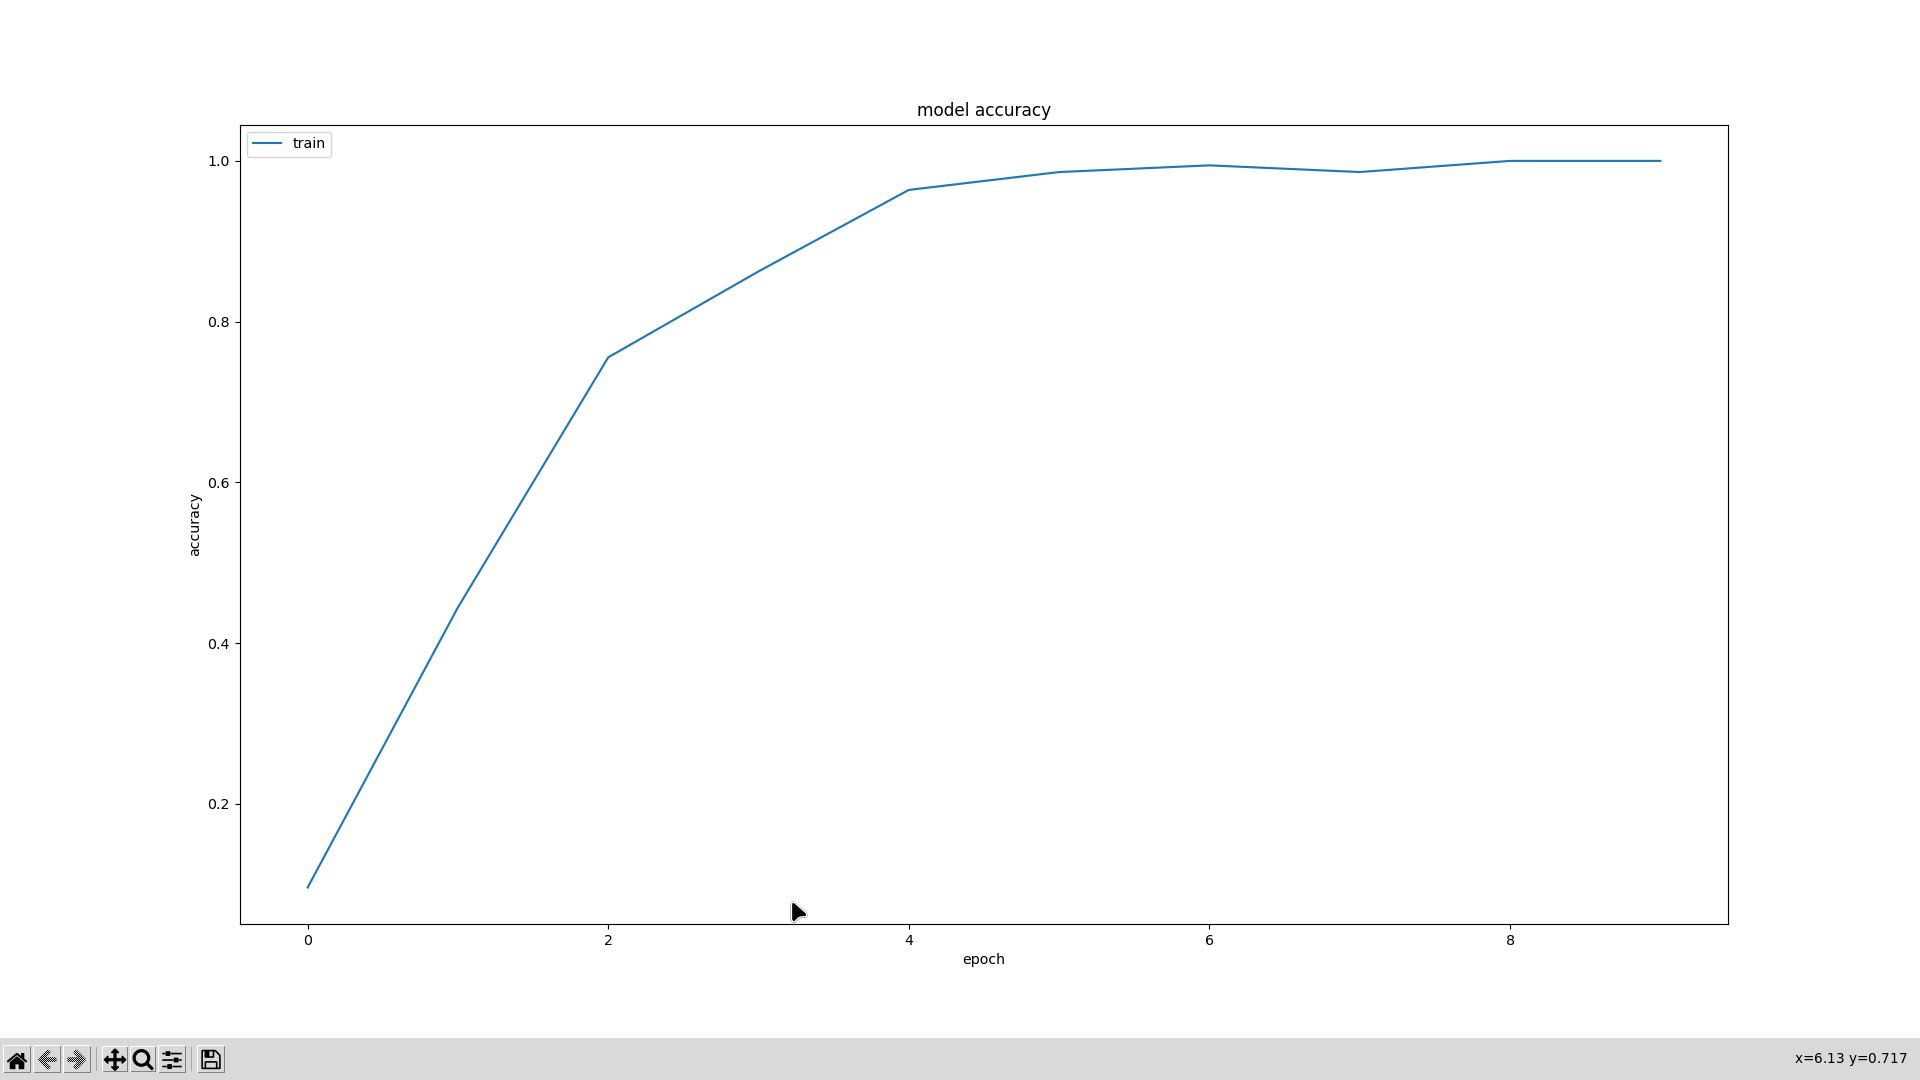
\includegraphics[scale=0.15]{neural_network_accuracy.png}}
	\caption{Neural Network model accuracy}
	\label{Neural_net_accuracy}
\end{figure}
\begin{figure}[htbp]
	\centerline{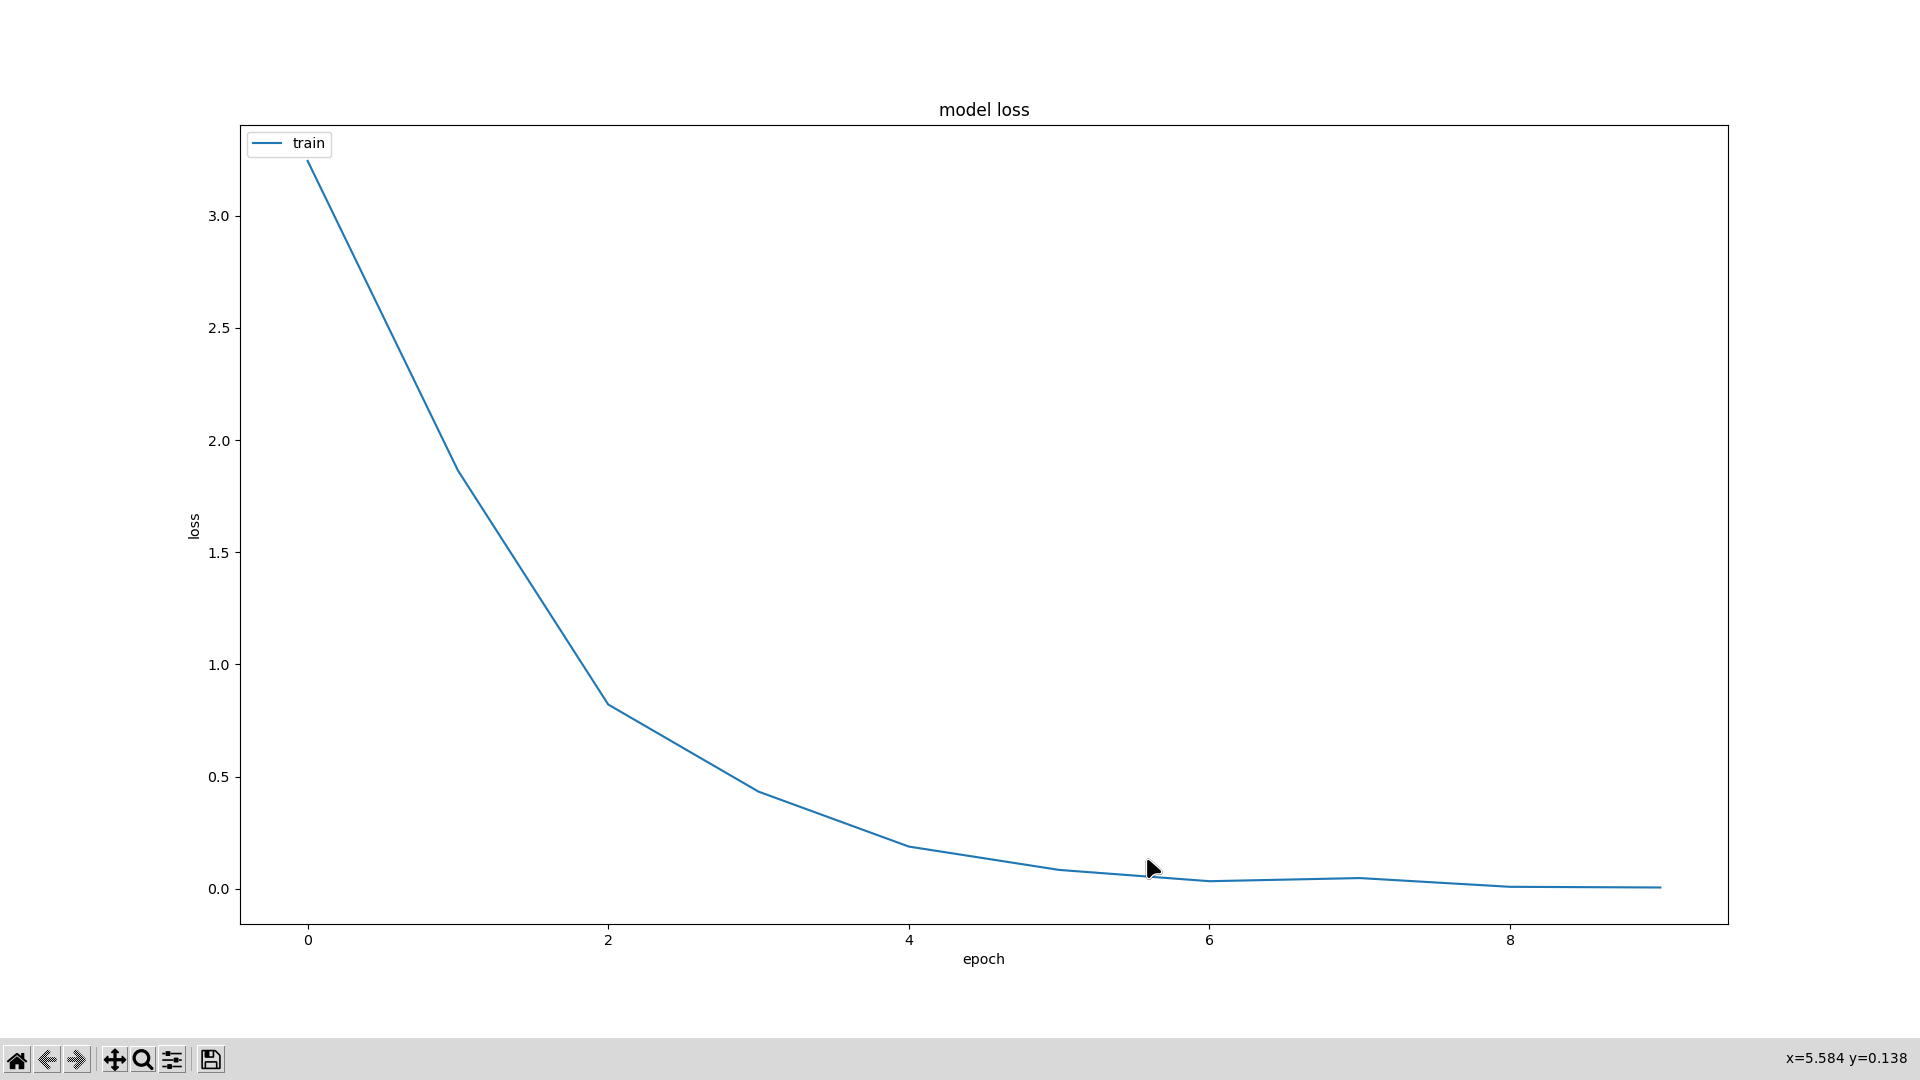
\includegraphics[scale=0.15]{neural_network_loss.png}}
	\caption{Neural Network model loss}
	\label{Neural_net_loss}
\end{figure}

\chapter{Merits, Limitations and Future Scope}

\section{Merits}
The merits of this architecture are:-
\begin{itemize}
	\item Really fast in terms of predictions and can be scaled to multiple users as the whole chatbot is dockerised and multiple containers can be spawned from the docker image.
	\item Also the final model used for predictions can be used to detect all ISL hand signs and it does that really fast.
	\item It can also detect characters with very complex hand signs very easily.
	\item Since we use a object detection framework like mediapipe, background color doesn't matter as long as mediapipe can detect the hands.
	\item Also relative positions of both hands with respect to each other and the other problem where the hand becomes bigger when near the webcam and small when farther from the webcam was addressed with the special preprocessing function which translates and transforms the hand coordinates to remove these issues.
	\item This whole architecture can be deployed on a normal server and still it can perform really well for multiple users upto a point because of the concept of multitasking implemented using goroutines and also the concept of mutex locks which allows the same model to be used by multiple users.
\end{itemize}

\section{Limitations}
The limitations of this project are:-
\begin{itemize}
	\item The dataset used to train the model is really small. It only has 20 samples representing each class. Because of this if the user shows a particular hand sign in a totally different way than the ones used in the dataset, we will not be able to predict it correctly.
	\item The dataset only consists of right handed samples. Left handed people presently cannot use this model for predictions. To do so they have to show the ISL hand signs as right handed people do.
	\item The dataset only consists of samples whose hands are small but if a person's hand is really large, then even though its coordinates are scaled to a range between 0 to 1, sometimes the predictions are false positive.
\end{itemize}


\section{Future Scope}
The future scope of this project is:-
\begin{itemize}
	\item The dataset used to train the working model is a really small dataset which only consists of 720 samples. Thus most of the limitations of this project are due to its small dataset size. If better dataset is used to train the model, We think it can become even more accurate at giving predictions in realtime with a webcam feed.
	\item We can train the model with left handed samples so as to make it predict ISL hand signs for left handed people as well.
	\item We can add a special custom hand sign for adding space in text so that word segmentation can be done even more accurately.
\end{itemize}

\chapter{Conclusion}
To summarize, ISL sign language detection is a key challenge in the field of AI(Artificial Intelligence) and ML(Machine Learning). We approached this problem in our own way using static image sign language recognition. So we take in a static image as input and then use this image to predict what ISL hand sign is shown in the image using various approaches. In the first approach, we trained a existing InceptionResnetV2 CNN model to detect the hand signs and predict the character of the 36 characters represented by the hand sign in the input image. This model when trained on the data set gave a really high accuracy of 98 percentile for both testing and training but failed to produce the same results in real time when deployed as the images in the data set had the hands as the main focus with dark and mono coloured background Also hand detection was required which was not done in this model. Most of all this model is really slow which is the biggest problem. So to approach this problem of better hand detection which the CNN model could not do, we used Mediapipe framework by google for hand coordinates detection in the image and then passed these coordinates to a custom preprocessed function which transforms and translates these coordinates to a range between 0 and 1 such that the relativity of positions of both the hands with respect to one another is removed and only shapes are considered. Now these processed coordinates are then passed to a neural network which used these coordinates to make a prediction as to which character was shown by the ISL sign in the image. This way, since Mediapipe could detect hands in wide variety of backgrounds and at any location in the image even though it is not the main focus, we resolved the previous problem which the CNN model had thus detecting hand signs in a variety of positions and lighting and even if the background is not mono coloured. Hence the model with mediapipe gave a better accuracy when deployed and could detect most of the hand signs very easily. Another catch to the mediapipe model is that it is very fast since very less computation is done than the CNN model which results in faster predictions. Finally we processed the model raw output using a bunch of techinques like taking maximum frequency element in a given sample, spellchecking and word segmentation to get the final predicted text.

\begin{thebibliography}{00}
	\bibitem{b1} Sign Language Recognition for Static and Dynamic Gestures by Jay Suthar
	\bibitem{b2} Zero-Shot Sign Language Recognition: Can Textual Data Uncover Sign Languages? by Yunus Can Bilge
	\bibitem{b3} A Review Paper on Sign Language Recognition of Engineering System For Deaf And Research \& Dumb People using Image Technology Processing by Manisha U. Kakde
	\bibitem{b4} Attention-Based Sign Language Recognition Network Utilizing Key frame Sampling and Skeletal Features by Wei Pan
	\bibitem{b5} Cooper, H., Holt, B. \& Bowden, R. Sign language recognition. In Visual Analysis of Humans, 539–562 (Springer, 2011).
	\bibitem{b6} Stergiopoulou, E., Sgouropoulos, K., Nikolaou, N., Papamarkos, N. \& Mitianoudis, N. Real time hand detection in a complex background. Engineering Applications of Artificial Intelligence 35, 54–70 (2014).
	\bibitem{b7} Aloysius, N. \& Geetha, M. A review on deep convolutional neural networks. In 2017 International Conference on Communication and Signal Processing (ICCSP), 0588–0592 (IEEE, 2017).
	\bibitem{b8} Nagi, J. et al. Max-pooling convolutional neural networks for vision-based hand gesture recognition. In Signal and Image Processing Applications(ICSIPA), 342–347 (IEEE, 2011).

	\bibitem{b9} Howard, A. G. et al. Mobilenets: Efficient convolutional neural networks for mobile vision applications. arXiv preprint arXiv:1704.04861 (2017).
	\bibitem{b10} von Agris, U., Blomer, C., Kraiss, K.F.: Rapid signer adaptation for continuous sign language recognition using a combined approach of eigenvoices, MLLR, and MAP. In: Procs. of ICPR, pp. 1 – 4. Tampa, Florida, USA (2008). DOI 10.1109/ICPR.2008.4761363
	\bibitem{b11} von Agris, U., Knorr, M., Kraiss, K.: The significance of facial features for automatic sign language recognition. In: Procs. of FGR, pp. 1 – 6. Amsterdam, The Netherlands (2008)
	\bibitem{b12} von Agris, U., Zieren, J., Canzler, U., Bauer, B., Kraiss, K.: Recent developments in visual sign language recognition. Universal Access in the Information Society 6(4), 323 – 362 (2008)
	\bibitem{b13} Akyol, S., Alvarado, P.: Finding relevant image content for mobile sign language recognition. In: Procs. of IASTEDInt. Conf. on Signal Processing, Pattern Recognition and Application, pp. 48 – 52. Rhodes, Greece (2001)
	\bibitem{b14} Aran, O., Burger, T., Caplier, A., Akarun, L.: A belief-based sequential fusion approach for fusing manual signs and non-manual signals. PATTERN RECOGN LETTERS 42(5), 812 – 822 (2009)
	\bibitem{b15} Athitsos, V., Sclaroff, S.: Estimating 3D hand pose from a cluttered image. In: Procs. of CVPR, vol. 2. Madison WI, USA (2003)
	\bibitem{b16} Awad, G., Han, J., Sutherland, A.: A unified system for segmentation and tracking of face and hands in sign language recognition. In: Procs. of ICPR, vol. 1, pp. 239 – 242. Hong Kong, China (2006). DOI 10.1109/ICPR.2006.194
	\bibitem{b17} Ba, S.O., Odobez, J.M.: Visual focus of attention estimation from head pose posterior proba- bility distributions. In: Procs. of IEEEInt. Conf. on Multimedia and Expo, pp. 53–56 (2008). DOI 10.1109/ICME.2008.4607369
	\bibitem{b18} Bailly, K., Milgram, M.: Bisar: Boosted input selection algorithm for regression. In: Procs. of Int. Joint Conf. on Neural Networks, pp. 249–255 (2009). DOI 10.1109/IJCNN.2009.5178908
	\bibitem{b19} Bauer, B., Hienz, H., Kraiss, K.: Video-based continuous sign language recognition using statistical methods. In: Procs. of ICPR, vol. 15, pp. 463 – 466. Barcelona, Spain (2000)
	\bibitem{b20} Bauer, B., Nießen, S., Hienz, H.: Towards an automatic sign language translation system. In: Procs. of Int. Wkshp : Physicality and Tangibility in Interaction: Towards New Paradigms for Interaction Beyond the Desktop. Siena, Italy (1999)
	\bibitem{b21} Bowden, R., Windridge, D., Kadir, T., Zisserman, A., Brady, M.: A linguistic feature vector for the visual interpretation of sign language. In: Procs. of ECCV, LNCS, pp. 390 – 401. Springer, Prague, Czech Republic (2004)
	\bibitem{b22} British Deaf Association: Dictionary of British Sign Language/English. Faber and Faber (1992)
	\bibitem{b23} Bungeroth, J., Ney, H.: Statistical sign language translation. In: Procs. of LREC : Wkshp : Representation and Processing of Sign Languages, pp. 105 – 108. Lisbon, Portugal (2004)
	\bibitem{b24} Coogan, T., Sutherland, A.: Transformation invariance in hand shape recognition. In: Procs. of ICPR, vol. 3, pp. 485 – 488. Hong Kong, China (2006). DOI 10.1109/ICPR.2006.1134
	\bibitem{b25} Cooper, H., Bowden, R.: Large lexicon detection of sign language. In: Procs. of ICCV : Wkshp : Human-Computer Interaction, pp. 88 – 97. Rio de Janario, Brazil (2007). DOI 10.1007/978-3-540-75773-3\ 10
\end{thebibliography}

\appendix
\chapter{Source Code}
You can access the source code from this link: \url{https://www.github.com/231tr0n/fyp}

\end{document}





















































































































































































































































































































































































































